Having successfully modeled our puzzle test-case using a Chemical
Reaction Network, we turn to the next step: Modifying this model so
that it behaves in a desired way.

This modification could be making it more efficient (i.e. optimizing
it for a given metric) or just attaining a specific goal (i.e.
create a specific final distribution). We define the control problem
as follows:
\begin{quote}
    Let a system of chemical reactions $R$, defined by a matrix of rate constants $K$, a stoichiometry
matrix $S$ and a vector of products and reactants $y$. Let the
initial condition $x_0$ be known also. What should be the matrix
$K_c$ so that the system converges as close as possible to a desired
equilibrium $\hat{X}$. Moreover, can we find the matrix $K_{f}$ that
converge as close as possible to $\hat{X}$ at the fastest rate?
\end{quote}

This is a design problem as well as an optimization problem. In the
second proposition, we are optimizing towards two different goals:
convergence and speed of convergence.

\section{Overview of possibilities} % (fold) \label{sec:overview_of_possibilities}

    Our first goal was to use a previous optimization scheme used by S. Berman~\cite{ref:BermanTRO08, Halasz:2007p10106}, namely optimizing the Mixing-time of a Markov chain~\cite{Randall:2006p11793, NEthier:1986p4833, Sun:2005p4975}. Unfortunately, our problem is not a Markov chain. Our model is a continuous-time Markov process, with nonlinear rates. Actually, it is possible to represent it as a Markov chain, an approach taken by Klavins for his optimization technique~\cite{Klavins:2007p2600}: we have to consider every possible macro-states or marking of the system starting from an initial condition, by discretizing all possible values taken by the products, and then creating or measuring the probabilities to jump from one macro-state to another. Obviously, this approach runs into a combinatorial explosion when the number of species and their populations increase, which forbids us from using it. Other approaches using Markov chains~\cite{Runolfsson:2007p9740, Tierney:1994p9783} are also abandoned because of this problem.

    Therefore, we looked into the chemical reaction networks literature for an optimization scheme taking advantage of the control we have on the stochastic constant rates.

    We found papers focusing on the reachability of networks, namely knowing what parts of the state space could be attained knowing the system dynamics~\cite{Berman:2007p10105, Bastin:1993p10351, Kloetzer:2006p9623, Bastin:1990p10531, Batt:2007p9650}. These works apply more to bioreactors and show little interest on the reaction rates.
    Other works, on the other hand, rely too much on a control theory methodology, for example by adding a feedback to the system~\cite{OteroMuras:2008p10653, Iglesias:2007p9153, Belta:2006p9642}. As we want to modify only the rates, these were not helpful.

    We found an interesting study in \cite{Schuster:1987p11838}. The authors propose an analysis and optimization of the rates of a chain of reactions, with respect to several objectives. Those objectives closely resembles the two propositions we are trying to solve, we will therefore use ideas from their work, although our approach is original. However, they are working with reaction chains, which offers simplifications and results that are not available for our more complex reaction network.

% section overview_of_possibilities (end)

\section{Methodology} % (fold) \label{sec:methodology}

    \subsection{Changes on our models} % (fold)
    \label{sub:changes_on_our_models}

        Starting from the chemical reaction network \eqref{eq:reaction_network_transportersimple}, we make several modifications in order to satisfy our methodology:

        \begin{my_enumerate}
            \item We remove the robots from the system. We assume that the number of robots is bigger or equal to the number of pieces and that the robots find and carry the piece very quickly with respect to the time between assemblies. Under those assumptions, we can remove the robots in a quasi steady-state assumption, looking only at the dynamics of the products.
            \item We add backward reactions to every existing assembling reaction. They correspond to the degradation of a product into its reactants. Such reactions are needed when we will prove that our new system has only one globally asymptotically stable equilibrium.
        \end{my_enumerate}

        The new chemical reaction network is:

        \begin{eqnarray}
            X_1 + X_2 ~~{\mathop{\rightleftharpoons}_{k_1^-}^{k_1^+}}~~ X_5 & \quad &  X_2 + X_7 ~~{\mathop{\rightleftharpoons}_{k_4^-}^{k_4^+}}~~ X_{F1} \nonumber \\
            X_3 + X_4 ~~{\mathop{\rightleftharpoons}_{k_2^-}^{k_2^+}}~~ X_6 & & X_2 + X_5 ~~{\mathop{\rightleftharpoons}_{k_5^-}^{k_5^+}}~~ X_8 \nonumber \\
            X_5 + X_6 ~~{\mathop{\rightleftharpoons}_{k_3^-}^{k_3^+}}~~ X_7 & & X_6 + X_8 ~~{\mathop{\rightleftharpoons}_{k_6^-}^{k_6^+}}~~ X_{F2}
            \label{eq:modified_system:reactions}
        \end{eqnarray}


        In the thermodynamic limit \cite{Gillespie:2007p1788}, the physical system represented by \eqref{eq:modified_system:reactions} can be abstracted to a linear ordinary differential equation (ODE) model:

        \begin{equation}\label{eq:ODEequations}
            \left\lbrace\begin{array}{lll}
                \dot{x}_1 &=& - k_1^+ x_1 x_2 + k_1^- x_5  \\
                \dot{x}_2 &=& - k_1^+ x_1 x_2 - k_5^+ x_2 x_5 - k_4^+ x_2 x_7 + k_1^- x_5 + k_{5}^- x_8 + k_4^- x_{F1}  \\
                \dot{x}_3 &=& - k_2^+ x_3 x_4 + k_2^- x_6 \\
                \dot{x}_4 &=& - k_2^+ x_3 x_4 + k_2^- x_6  \\
                \dot{x}_5 &=&   k_1^+ x_1 x_2 - k_1^- x_5 - k_3^+ x_5 x_6 + k_3^- x_7 - k_5^+ x_2 x_5 + k_{5}^- x_8  \\
                \dot{x}_6 &=&   k_2^+ x_3 x_4 - k_2^- x_6 - k_3^+ x_5 x_6 + k_3^- x_7 - k_{6}^+ x_6 x_8 + k_{6}^- x_{F2} \\
                \dot{x}_7 &=&   k_3^+ x_5 x_6 - k_3^- x_7 - k_4^+ x_2 x_7 + k_4^- x_{F1} \\
                \dot{x}_8 &=&   k_5^+ x_2 x_5 - k_{5}^- x_8 - k_{6}^+ x_6 x_8 + k_{6}^- x_{F2} \\
                \dot{x}_{F1} &=& k_4^+ x_2 x_7 - k_4^- x_{F1} \\
                \dot{x}_{F2} &=& k_{6}^+ x_6 x_8 - k_{6}^- x_{F2}
            \end{array}
            \right.
        \end{equation}

        Define a matrix $\mathbf{M} \in \mathbb{R}^{10 \times 12}$ in which
        each entry $m_{ji}$, $j=1,...,10$, of column $\mathbf{m}_i$ is
        defined as the coefficient of piece type $j$ in complex $i$ ($0$ if
        the piece type is absent).  For instance, the column corresponding
        to the complex $X_1 + X_2$ is $[1~1~0~0~0~0~0~0~0~0]^T$.  Now
        represent the rate associated with reaction $(i,j) \in \mathcal{E}$
        as $k_{ij}$ and define a matrix $\mathbf{K} \in \mathbb{R}^{12
        \times 12}$ with entries:

        \begin{equation}
            K_{ij} =  \left\{
                \begin{array}{lll}
                    k_{ji} &\mbox{ if }& i \neq j~, ~~(j,i) \in \mathcal{E}~, \\
                    0 &\mbox{ if }& i \neq j~, ~~(j,i) \notin \mathcal{E}~,\\
                    -\sum_{(i,l)\in {\mathcal E}} k_{il} &\mbox{ if }& i=j~.
                \end{array} \right. \label{eq:Kdef}
        \end{equation}

        Finally, define a vector $\mathbf{y(x)} \in \mathbb{R}^{12}$ in
        which entry $y_i$ is the piece variable or products of variables
        associated with complex $i$:

        \begin{equation} \mathbf{y(x)} = [x_1
            x_2~~x_5 ~~x_3 x_4 ~~x_6 ~~x_2 x_7 ~~x_{F1}~~x_5 x_6~~ x_7~~x_2 x_5
            ~~x_8~~ x_6 x_8 ~~x_{F2}]^T~. \label{eq:ydef1}
        \end{equation}

        Then the ODE model \eqref{eq:ODEequations} can be written in the
        following form \cite{Chaves:2004p11839}:

        \begin{equation}
            \mathbf{\dot{x}} = \mathbf{M}\mathbf{K}\mathbf{y}(\mathbf{x})~,
            \label{eq:matrixODE}
        \end{equation}

        One set of conservation constraints on the piece quantities is:
        \begin{equation}
            \left\lbrace
                \begin{array}{lll}
                    x_3 - x_4 &=& N_1 \\
                    x_1+x_5+x_7+x_8+x_{F1}+x_{F2} &=& N_2 \\
                    x_2+x_5+x_7+2(x_8+x_{F1}+x_{F2}) &=& N_3 \\
                    x_3+x_6+x_7+x_{F1}+x_{F2} &=& N_4
                \end{array}
            \right.
            \label{eq:cons}
        \end{equation}
        where $N_i$, $i=1,...,4$, are computed from the initial piece
        quantities.

        We will study this network from now on.
    % subsection changes_on_our_models (end)

    \subsection{Approach} % (fold)
    \label{sub:approach}
        Our optimization relies on the following hypotheses:

        \begin{my_enumerate}
            \item The system \eqref{eq:matrixODE} is deterministic and its dynamics depend only on the rates $\mathbf{K}$ and the initial conditions.
            \item The system, while nonlinear in $x_i$, converge to an unique positive equilibrium given an initial condition and a matrix $\mathbf{K}$.
            \item The system \eqref{eq:matrixODE} is nonlinear in $x_i$ but linear in $k_i$.
            \item $\mathbf{K}$ governs the rate of convergence of the system.
            \item $\mathbf{M}\mathbf{K}\mathbf{y}(\mathbf{x}) = 0$ only at the equilibrium point.
        \end{my_enumerate}

        Hypothesis 1 derives from the definition of an ODE and on the fact that we keep the network fixed during the system evolution. Hypothesis 2 will be proved in Section~\ref{sub:convergence_of_chemical_reaction_networks}, it is a main result in the success of our approach. Hypothesis 3 comes from the observation of the system \eqref{eq:ODEequations}. Hypothesis 4 will be discussed in Section~\ref{sub:design_of_optimal_rates}. Hypothesis 5 is discussed in Section~\ref{sub:design_of_optimal_rates}.

        Then, under those hypothesis, it is possible to find an objective function linear in $k_i$, using $\mathbf{M}\mathbf{K}\mathbf{y}(\mathbf{x^d}) = 0$ as a set of constraints on the desired converged values of $x^d$ and solve it using a convex optimization algorithm.

        The complete derivation and discussion is presented in Section~\ref{sub:design_of_optimal_rates}.

    % subsection approach (end)

    \subsection{Convergence of chemical reaction networks} % (fold)
    \label{sub:convergence_of_chemical_reaction_networks}

        \begin{theorem}\label{thm:unique_equilibrium}
        System \eqref{eq:ODEequations} subject to \eqref{eq:cons} has a
        unique equilibrium $\mathbf{\bar{x}} > \mathbf{0}$.
        \end{theorem}

        \begin{proof}

        Each steady state of the system can be classified
        as either a {\it positive} steady state, $\{ \mathbf{\bar{x}}
        ~|~\mathbf{M}\mathbf{K}\mathbf{y(\bar{x})} = \mathbf{0}, ~\bar{x}_i
        0~\forall i\}$, or a {\it boundary} steady state, $\{ \mathbf{\bar{x}}
        ~|~\mathbf{M}\mathbf{K}\mathbf{y(\bar{x})} = \mathbf{0}, ~\bar{x}_i
        = 0 \mbox{ for some } i\}$, which can be found by solving
        $\mathbf{y(\mathbf{\bar{x}})} = \mathbf{0}$~\cite{Chaves:2004p11839}.

        From definition \eqref{eq:ydef1} of $\mathbf{y(x)}$, the boundary
        steady states for the system satisfy

        \begin{eqnarray}
        \bar{x}_5 = \bar{x}_6 = \bar{x}_7 = \bar{x}_8 = \bar{x}_{F1} =
        \bar{x}_{F2} = 0~, \nonumber \\
        \bar{x}_1 \bar{x}_2 = \bar{x}_3 \bar{x}_4 = \bar{x}_2 \bar{x}_7=
        \bar{x}_5 \bar{x}_6 = \bar{x}_2 \bar{x}_5 = \bar{x}_6 \bar{x}_8 =
        0~.
        \end{eqnarray}
        It can be concluded that in each boundary steady state, all $x_i =
        0$ except for one of the four combinations of variables $(x_1,x_3),
        (x_1,x_4), (x_2,x_3), (x_2,x_4)$.  Since we only consider systems
        that can produce $x_{F1}$ and $x_{F2}$, it is not possible for the
        system to reach any of these steady states; each one lacks two piece
        types needed for the final assemblies.

        The {\it deficiency} $\delta$ of a reaction network has been introduced
        as a measure giving insights and proofs on the stability and the existence of equilibrium of a class of reaction networks \cite{Feinberg:1987p9428, Craciun:2005p10148, Craciun:2006p9417, Feinberg:1995p9419, Feinberg:1997p9425, Bernstein:1999p10604, Craciun:2006p10142}. It is one of the two attempts at proving convergence and stability of chemical reaction network, the other one is based on so-called species-reaction graphs analysis \cite{Sontag:2007p9303, Angeli:2008p9287, Sontag:2004p9319, Chaves:2004p9259, Sontag:2001p9286}.

        $\delta$ is calculated has the number of complexes minus the number of {\it linkage classes}, each of which
        is a set of complexes connected by reactions, minus the network {\it
        rank}, which is the rank of the matrix whose rows are each obtained
        by subtracting a column of $\mathbf{M}$ associated with a reactant
        in a particular reaction from a column associated with a product
        \cite{Feinberg:1987p9428}.  It can be shown that each of the six
        linkage classes in our system has rank $1$ and the rank of the
        entire network is $6$; from this the deficiency of each linkage
        class is calculated to be $0$ and the deficiency of the entire
        network is $0$ as well. Also, we observe that no complex in any
        linkage class transforms into a complex in another linkage class.
        These properties, along with the fact that the system kinetics are
        mass-action, satisfy the criteria for applying the Deficiency One
        Theorem in \cite{Feinberg:1987p9428}, which gives the result that
        the system can have no more than one positive steady state.

        Now we must show that there exists a positive steady state, which
        would be unique by the Deficiency One result.  Since the network
        rank of the system is the sum of the ranks of the linkage classes,
        the linkage classes constitute a {\it direct partition} of the
        network \cite{Feinberg:1995p9419}.  Also, since each linkage class
        has deficiency $0$ and is {\it weakly reversible}, meaning that
        there is a reaction pathway connecting each pair of complexes, each
        linkage class contains exactly one positive steady state by the
        Deficiency Zero Theorem \cite{Feinberg:1987p9428}.  By Lemma 8.2.3
        of \cite{Feinberg:1995p9419}, these properties imply that the system
        admits a positive steady state.

        \end{proof}

        We still lack a proof on the stability of this unique equilibrium. If the deficiency zero theorem \cite{Feinberg:1987p9428} can be extended to support not only \textit{weakly reversible} but also \textit{block weakly reversible} networks, than we would get that results. A remark in \cite{Chaves:2004p9259} support that fact, but we did not manage to get a formal result as of today. However, the empirical experiments we are doing show that the equilibrium is stable, so we will assume this fact from now on.
    % subsection convergence_of_chemical_reaction_networks (end)

    \subsection{Design of optimal rates} % (fold)
    \label{sub:design_of_optimal_rates}

        We consider the problem of designing the assembly system
        described by model \eqref{eq:ODEequations} subject to
        \eqref{eq:cons} to produce desired quantities of pieces. The derivation is similar for other systems.

        \subsubsection{System and equilibrium definition} % (fold)
        \label{ssub:system_and_equilibrium_definition}
        The assembly system will be most productive if it yields the target
        quantities as quickly as possible.  This objective will be posed as
        the design of a set of {\it optimal rates} $k_i^+, k_i^-$, $i=1,...,6$, for
        model \eqref{eq:ODEequations} that minimizes the convergence time
        of the resulting system to a target vector of piece quantities,
        $\mathbf{x^d}$.

        Note that although the quantities of only the final
        assemblies, $X_{F1}$ and $X_{F2}$, may need to be specified in
        practice, the optimization problem requires that target quantities
        of intermediate components be defined as well, as will be discussed
        later in this section.

        The rates $k_i^+, k_i^-$ can be chosen so that the assembly system yields a
        target piece distribution $\mathbf{x^d}
        > \mathbf{0}$ starting from {\it any} initial distribution of
        pieces:

        \begin{my_enumerate}
            \item First, specify target numbers of the intermediate and final assemblies, $x_i^d$, $i=5,...,8$.
            \item Then define piece quantities $x_j^d$, $j=1,...,4$, in terms of these numbers according to the conservation equations \eqref{eq:cons}.
            \item Finally define $\mathbf{y^d} = \mathbf{y(x^d)}$ according to definition \eqref{eq:yExp}.
        \end{my_enumerate}

        This vector $y^d$ represents the steady-state quantities of the pieces and piece products associated with each complex.
        If the system described in the form \eqref{eq:matrixODE} converges to $\mathbf{y^d}$, then it converges to the
        target quantities $x_i^d$, $i=5,...,8$, since eight components of
        $\mathbf{y^d}$ are equal to these variables. Convergence to $x_j^d$, $j=1,...,4$ is also ensured since each of these quantities is a
        function of $x_i^d$, $i=5,...,8$ by conservation laws.

        By Theorem \ref{thm:unique_equilibrium}, model \eqref{eq:ODEequations} always converges to a single positive
        equilibrium $\mathbf{\bar{y}}$. Therefore, system convergence to
        $\mathbf{y^d}$ can be guaranteed by specifying that
        $\mathbf{\bar{y}} \equiv \mathbf{y^d}$ through the following
        constraint on the rate matrix $\mathbf{K}$ in model \eqref{eq:matrixODE}:

        \begin{equation}
            \mathbf{M}\mathbf{K}\mathbf{y^d} = \mathbf{0}~.
            \label{eq:equilConstr}
        \end{equation}

        To control more easily the goal in term of final puzzles, we introduce the fraction $\alpha$:
        \begin{equation} \label{eq:alpha}
            \alpha = \frac{x_{F1}}{x_{F1}+x_{F2}}
        \end{equation}
        The target final assemblies can be defined in such a way that their
        sum, $x_{F1}+x_{F2}$, is constant and the fraction $\alpha$ is directly a tunable parameter. The sum
        $x_{F1}+x_{F2}$ is expressed in terms of a conservation law, which
        means that one of the target quantities $x_i^d$, $i \in
        \{1,...,4\}$, must be implicitly defined. For instance, using the
        second conservation equation in \eqref{eq:cons} and a target
        value for $x_2^d$:

        \begin{eqnarray}
            x_{F1}^d &=& \tfrac{1}{2}~ \alpha ~\left(N_2-(x_2^d+x_5^d+x_7^d+2 x_8^d)\right)~ \\
            x_{F2}^d &=& \tfrac{1}{2}~ (1-\alpha) ~\left(N_2-(x_2^d+x_5^d+x_7^d+2 x_8^d)\right)~,
        \end{eqnarray}

        Whatever the selection of independent piece quantities, it must be
        ensured that the remaining piece quantities are positive to have a
        feasible $\mathbf{x^d}$ (positive equilibrium).

        % subsubsection system_and_equilibrium_definition (end)

        \subsubsection{Convergence time} % (fold)
        \label{ssub:convergence_time}

        Now we consider the aspect of minimizing the convergence time of the
        system to the target equilibrium $\mathbf{x^d}$.  We can define
        measures of this time by reformulating the system in terms of new
        variables.  Define $v_j$, $j=1,...,6$, as the difference between
        the forward and reverse fluxes associated with reaction $j$ in
        system \eqref{eq:modified_system:reactions}.

        For instance, if we label reaction $1$ as the one in which $X_1 + X_2$ is the
        reactant and $X_5$ is the product, then $v_1 = k_1 x_1 x_2 - k_2
        x_5$.  Let $\mathbf{v(x)} = [v_1~...~v_{6}]^T$.  Denote the
        stoichiometric matrix of the system by $\mathbf{S} \in
        \mathbb{R}^{6 \times 10}$, which is defined such that model
        \eqref{eq:ODEequations} can be written as \cite{bib:Heinrich1996}:

        \begin{equation}
            \mathbf{\dot{x}} = \mathbf{S} \mathbf{v(x)}~.
        \end{equation}

        %The entries $s_{ij}$ of $\mathbf{S}$ for this model are $-1$, $0$,
        %or $1$.

        Our assembly system is similar to a model of a biochemical network
        with mass action kinetics.  The dynamical properties of such
        networks are often analyzed by linearizing the ODE model of the
        system about a steady state and studying the properties of the
        associated Jacobian matrix $\mathbf{J} = \mathbf{S} \mathbf{G}$,
        where the entries of $\mathbf{G}$ are $g_{ij} = dv_i/dx_j$ (see
        \cite{bib:Jamshidi2008} for an overview and further references).

        Denoting the eigenvalues of $\mathbf{J}$ by $\lambda_i$, $\tau_i =
        1/|Re(\lambda_i)|$ are measures of the characteristic times,
        referred to as {\it relaxation times}, in which different modes
        (dynamically independent variables) of the the system converge to a
        stable steady state after perturbation~\cite{bib:Heinrich1977, bib:Jamshidi2008}.

        Since the $\lambda_i$ are negative at a stable steady state, one way to yield fast convergence is to choose
        rates $k_i$ that minimize the largest $\lambda_i$, as was done for a
        linear chain of enzymatic reactions in~\cite{Schuster:1987p11838}.

        However, in our system it is very difficult to find analytical
        expressions for the $\lambda_i$, so we must explore other ways of
        quantifying the convergence time.

        Various measures of average relaxation times in biochemical networks
        have been defined, but they are applicable only under certain
        conditions, such as a linear reaction sequence
        \cite{bib:Heinrich1991}.  For instance, one such measure was
        minimized in the optimization of rates for the linear chain in
        \cite{Schuster:1987p11838}.  For our system, we can use a general
        estimate of the relaxation time for each reaction $j$ that is given
        in \cite{bib:Heinrich1996}.  It is derived by linearizing the system
        model around its equilibrium point, which in our case is the target
        distribution $\mathbf{x^d}$ enforced by equation~\eqref{eq:equilConstr}:

        \begin{equation}
        \tau_j = \left( \sum_{i=1}^{12} (-s_{ij}) \frac{d v_j}{d x_i}
        \right)^{-1} \label{eq:tau}
        \end{equation}

        This expression is evaluated at $\mathbf{x^d}$.
        Since each reaction $j$ in system \eqref{eq:modified_system:reactions} is of
        the form $X_k + X_l
        ~~{\mathop{\rightleftharpoons}_{k_j^-}^{k_j^+}}~~ X_m$, the net flux
        $v_j$ is $k_j^+ x_k x_l - k_j^- x_m$, and the entries of column $j$
        in $\mathbf{S}$ are all $0$ except for $s_{kj} = s_{lj} = -1$ and
        $s_{mj} = 1$. Thus, according to equation \eqref{eq:tau}, the
        relaxation time for each reaction is

        \begin{equation}
            \tau_j = (k_j^+(x_k^d + x_l^d) + k_j^-)^{-1}~. \label{eq:tauSys}
        \end{equation}

        This could give us a measure of speed of convergence.

        % subsubsection convergence_time (end)

        \subsubsection{Objective functions} % (fold)
        \label{ssub:objective_functions}

        Define $\mathbf{k} \in \mathbb{R}^{12}$ as the vector of all rates
        $k_i^+, k_i^-$. Using characterization \eqref{eq:tauSys} of reaction
        relaxation times, we define two possible objective functions
        $f:\mathbb{R}^{12} \rightarrow \mathbb{R}$ to {\it maximize} in
        order to produce fast convergence to $\mathbf{x^d}$.

        The first is the average inverse relaxation time,

        \begin{equation}
            f_{ave}(\mathbf{k}) = \tfrac{1}{10} \sum_{j=1}^{10} \tau_j^{-1}~.
        \end{equation}

        The second is the minimum inverse relaxation time,

        \begin{equation}
            f_{min}(\mathbf{k}) = \min \{ \tau_1^{-1}, \ldots, \tau_{10}^{-1}\}~.
        \end{equation}

        % subsubsection objective_functions (end)

        \subsubsection{Convex program definition} % (fold)
        \label{ssub:convex_program_definition}

        Finally, we map the rates onto actual adjustable parameters of the physical
        assembly system. Those adjustable parameters will be defined as the optimization variables.

        \begin{description}
            \item[Backward rates] Each reverse rate $k_j^-$ will be defined simply as a probability
            per unit time of breaking up an assembly, $p_j^- \in \{0, 1\}$, which can be
            adjusted:
            \begin{equation} \label{eq:backward_rate_opt}
                k_j^- = p_j^-
            \end{equation}
            \item[Forward rates] We use the formula \eqref{eq:reaction_assembly_rate} defined in Section~\ref{sub:theoretical_value_of_reaction_rates}. We extend it by adding a probability of starting the assembly $p_j^+  \in \{0, 1\}$ which can be adjusted:
            \begin{equation} \label{eq:forward_rate_opt}
                k_j^+ = p^e_j \cdot p^a_j \cdot p_j^+
            \end{equation}
            $p_j^e$ is the encountering probability defined by \eqref{eq:encountering_probability}, dependent on some parameters and $p_j^a$ is the assembly success rate, which we measure as explained in Section~\ref{ssub:stochastic_constant_rates_values}.
        \end{description}

        Let $\mathbf{p} \in \mathbb{R}^{12}$ be the vector of all adjustable
        probabilities, $p_j^+$ and $p_j^-$. Then we define an optimization Problem P as follows:

        \paragraph{P:} ~maximize ~~ $f(\mathbf{k(p)})$

        \vspace{1.5mm}

        \hspace{2.5mm} subject to ~~$\mathbf{M}\mathbf{K(p)}\mathbf{y^d} =
        \mathbf{0}$, ~~$\mathbf{0} \leq \mathbf{p} \leq \mathbf{1}$~.
        \vspace{2mm}

        % paragraph p1_ (end)

        \noindent Depending on the objective function used, we define Problem P1 and Problem P2:

        \paragraph{P1:} ~maximize ~~ $f_{ave}(\mathbf{k(p)})$

        \vspace{1.5mm}

        \hspace{4.5mm} subject to ~~$\mathbf{M}\mathbf{K(p)}\mathbf{y^d} =
        \mathbf{0}$, ~~$\mathbf{0} \leq \mathbf{p} \leq \mathbf{1}$~.
        \vspace{2mm}

        % paragraph p1_ (end)

        \paragraph{P2:} ~maximize ~~ $f_{min}(\mathbf{k(p)})$

        \vspace{1.5mm}

        \hspace{4.5mm} subject to ~~$\mathbf{M}\mathbf{K(p)}\mathbf{y^d} =
        \mathbf{0}$, ~~$\mathbf{0} \leq \mathbf{p} \leq \mathbf{1}$~.
        \vspace{2mm}

        % paragraph p1_ (end)

        Since this problem can be formulated as the minimization of a linear
        combination of the entries of $\mathbf{p}$ subject to a set of
        linear equality and inequality constraints on $\mathbf{p}$, it is a
        linear program, which can be solved efficiently.

        % subsubsection convex_program_definition (end)

    % subsection design_of_optimal_rates (end)

    \subsection{Optimization implementation} % (fold)
    \label{sub:optimization_implementation}
        In order to optimize the convex programs P1 and P2, we use a framework for Matlab, YALMIP\cite{Lofberg:2004p11461}. It allows us to define our optimization variables, objective function and constraints and to apply a semidefinite programming solving algorithm, running in polynomial time \cite{Lofberg:2004p11461}.
    % subsection optimization_implementation (end)
% section methodology (end)



\section{Results and limitations} % (fold)
\label{sec:results_and_limitations}

    We start with problem P1, which uses the first objective function $f_{ave}$, optimizing the average inverse relaxation time. We take the system \eqref{eq:modified_system:reactions} and optimize it according to our methodology:

    \begin{my_itemize}
        \item As discussed in Section~\ref{sub:experiment_3_5_pieces_and_5_robots_final_puzzles_f1_and_f2}, we use an initial condition with a big copy number of pieces, to avoid convergences problems: we use 60 pieces \{1, 3, 4, 5\}, 120 pieces 2 and no other mid-assemblies.
        \item For the forward rates, we assume that we can only optimize the probability of starting an assembly, $p_j^+$. This probability comes in addition to the probability of encounter and the probability of successful assembly, as shown in Equation~\eqref{eq:forward_rate_opt}. It can take values from $0$ to $1$.
        \item For the backward rates, we optimize the probability of breaking up an assembly $p_j^-$, as Equation~\eqref{eq:backward_rate_opt}. It can take values from $0$ to $1$.
        \item Our goal is to control the ratio $\alpha$ between the final number of F1 and F2 puzzles, Equation~\eqref{eq:alpha}. The converged number of other pieces are set to the smaller values still consistent with conservation laws and non-negativity constraints.
    \end{my_itemize}

    We optimize the system for every $\alpha \in {0.01, 0.99}$ and store the obtained rates for all 6 reactions.

    It turns out that nearly all rates keep constant values. All the forward rates are put to their maximal values. Backward rates all take constant positive values, except the backward rates of reactions 4 and 6, which vary continuously with respect to $\alpha$. Table~\ref{tab:optimized_rates_p1} resumes the situation.

    \begin{table}
        \begin{center}
        \begin{tabular}{|c|c|c|c|c|c|c|}
            \hline
            \textbf{Reaction} $\mathbf{j}$ & \textbf{1} & \textbf{2} & \textbf{3} & \textbf{4} & \textbf{5} & \textbf{6} \\
            \hline
            \textbf{Optimized} $\mathbf{p^+_j}$ & \multicolumn{6}{c|}{1.0} \\
            \hline
            \textbf{Optimized} $\mathbf{p^-_j}$ & 0.01885 & 0.00754 & 0.00377 & \textit{continuous} & 0.00942 & \textit{continuous} \\
            \hline
        \end{tabular}
        \end{center}
        \caption{Values of optimized rates for varying $\alpha$, under objective function P1.}
        \label{tab:optimized_rates_p1}
    \end{table}

    The case of the continuously varying rates is very interesting. Those rates corresponds to the backward reaction coming from the two final puzzles F1 (reaction 4) and F2 (reaction 6). Their evolution with respect to $\alpha$ is shown in Figure~\ref{fig:img_optimized_rates_alpha_p1}.

    \begin{figure}[h]
        \centering
            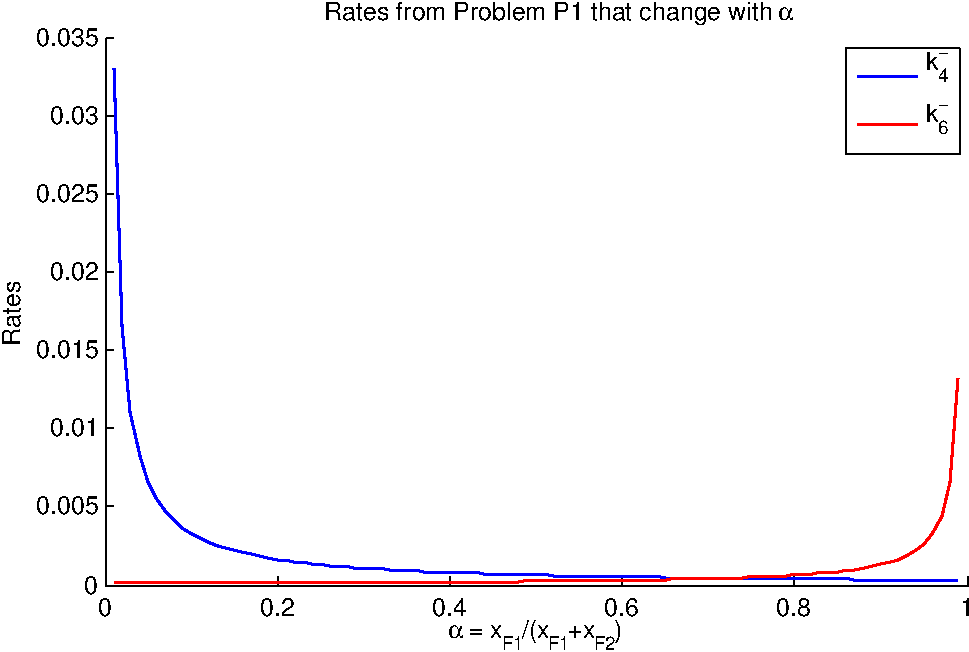
\includegraphics[width=10cm]{img/optimized_rates_alpha_p1.pdf}
        \caption{Backward rates changing continuously with respect to $\alpha$ under objective function P1.}
        \label{fig:img_optimized_rates_alpha_p1}
    \end{figure}

    Having constant rates for every reaction except those two give several informations:

    \begin{my_itemize}
        \item The network is highly flexible, allowing every ratio of final puzzles only by changing two specific backward rates. The non final reactions are kept to an activity low enough so as not to destroy to yield, but still high enough to be able to redistribute the materials when the final reactions are breaking up to converge to a desired ratio. Controlling only the disassembly rate of the two final puzzles is enough to attain any ratio $\alpha$, while optimizing the yield and time to convergence.
        \item All the forward rates are put to their maximum value. This could show that using non-maximum forward rates decreases the convergence rate, but further tests about that hypothesis are necessary.
    \end{my_itemize}

    Doing the optimization of problem P2, under objective function $f_{min}$ leads to slightly different results. This time the forward rates and backwards rates of reactions 4 and 6 are varying continuously. The forwards rate are not all maximum. Table~\ref{tab:optimized_rates_p2} presents the results for P2.

    \begin{table}
        \begin{center}
        \begin{tabular}{|c|c|c|c|c|c|c|}
            \hline
            \textbf{Reaction} $\mathbf{j}$ & \textbf{1} & \textbf{2} & \textbf{3} & \textbf{4} & \textbf{5} & \textbf{6} \\
            \hline
            \textbf{Optimized} $\mathbf{p^+_j}$ & 0.36 & 0.666 & 1.0 & \textit{continuous} & 0.4705 & \textit{continuous}\\
            \hline
            \textbf{Optimized} $\mathbf{p^-_j}$ & 0.006855 & 0.005027 & 0.00377 & \textit{continuous} &  0.00443 & \textit{continuous} \\
            \hline
        \end{tabular}
        \end{center}
        \caption{Values of optimized rates for varying $\alpha$, under objective function P2.}
        \label{tab:optimized_rates_p2}
    \end{table}

    Again with that objective function, the real control of the ratio $\alpha$ is carried on by the last two reactions in the construction of the final assemblies. This time the forward rates have a stronger role in that, but this has yet to be verified that this method is better. See Figure~\ref{fig:img_optimized_rates_alpha_p2} for the continuous variation of rates with respect to $\alpha$.

    \begin{figure}[h]
        \centering
            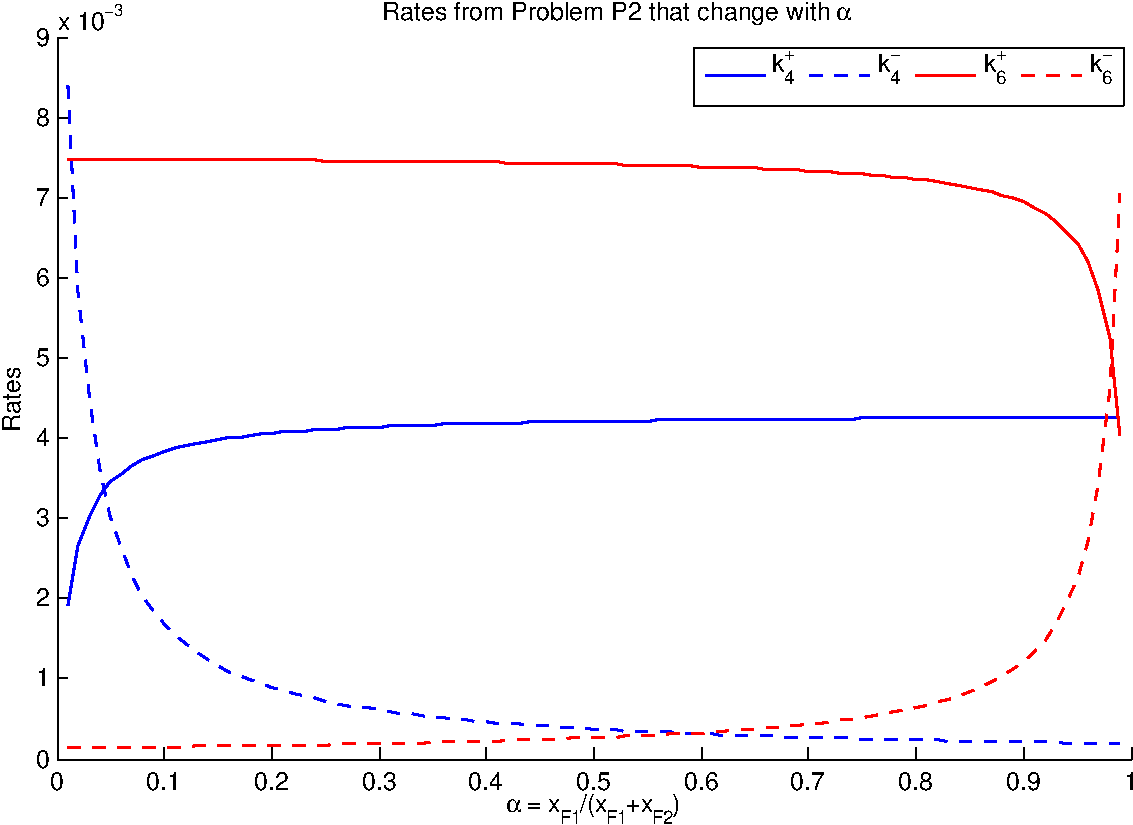
\includegraphics[width=10cm]{img/optimized_rates_alpha_p2.pdf}
        \caption{Forward and backward rates changing continuously with respect to $\alpha$ under objective function P2.}
        \label{fig:img_optimized_rates_alpha_p2}
    \end{figure}

    \subsection{Comparison between objective functions and strategies} % (fold)
    \label{sub:comparison_between_objective_functions_and_strategies}

        To compare the two functions, we plot the time-evolution of the ratio of the final puzzles F1 and F2 for three different $\alpha$: $0.1$, $0.5$ and $0.9$, see Figure~\ref{fig:optim_objfct_comparison} a-c). The horizontal dotted lines show the target ratios and both objective function are shown (plain for P1, dashed for P2).

        \begin{figure}[h!]
            %\centering
            \subfigure[$\alpha = 0.1$, Linear x axis.]
            {
                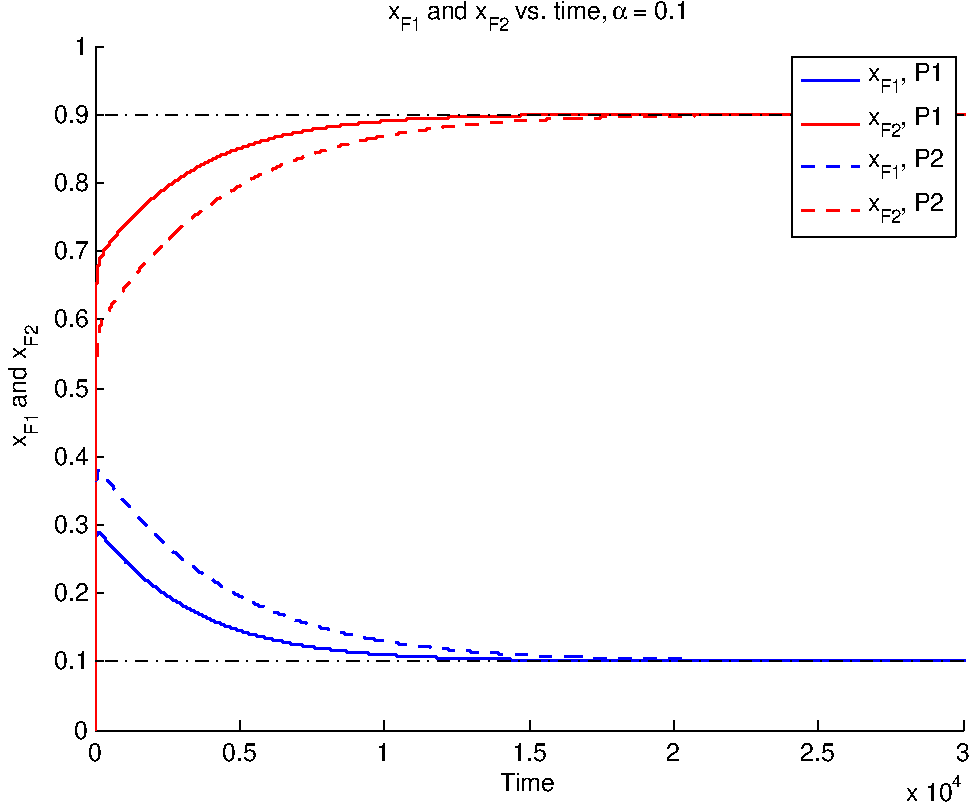
\includegraphics[width=7.2cm]{img/optim_conv_alpha01_lin.pdf}
                \label{fig:optim_objfct_comparison:alpha01_lin}
            }
    %       \: % espacement entre figures. \quad \;
            \subfigure[$\alpha = 0.1$, Log x axis.]
            {
                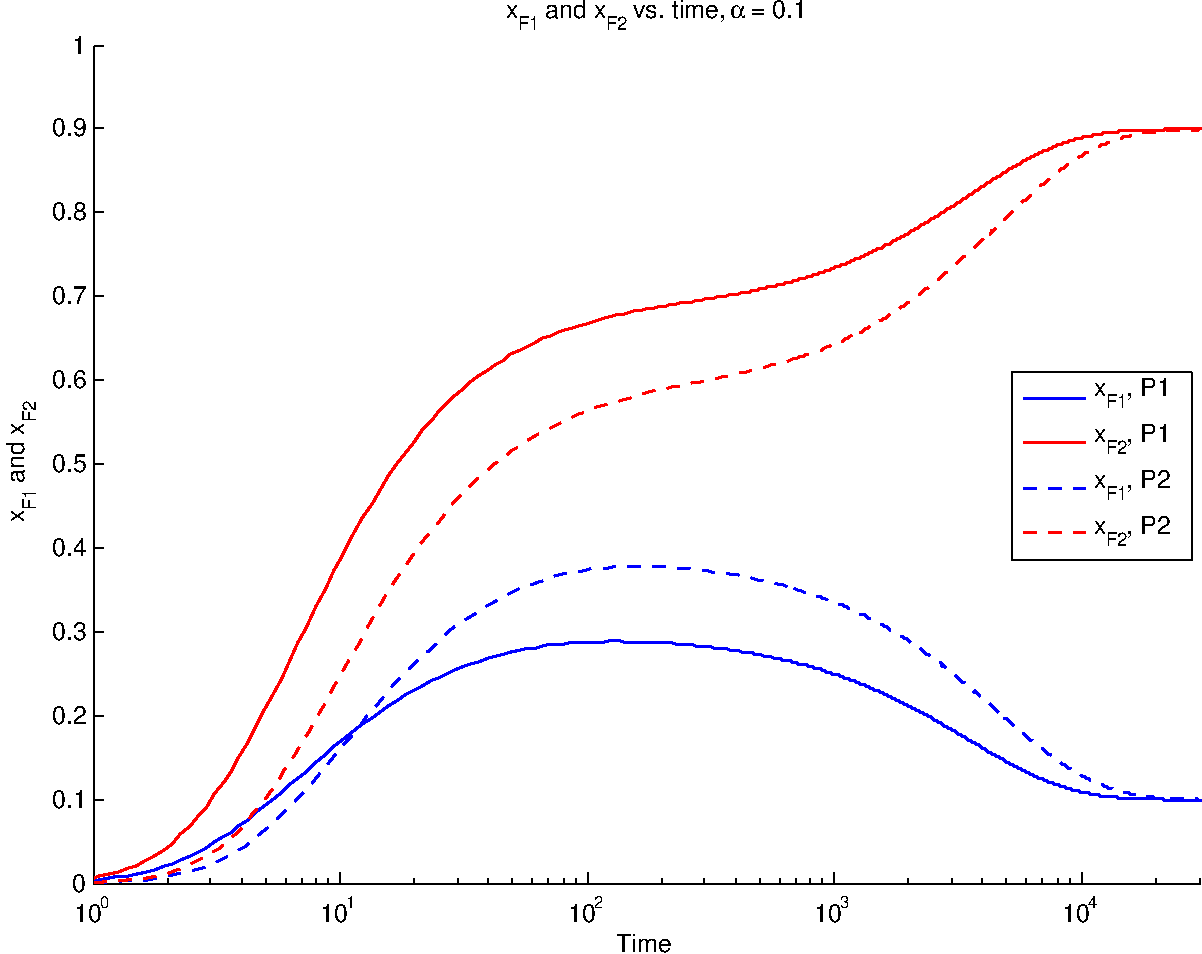
\includegraphics[width=7.2cm]{img/optim_conv_alpha01_log.pdf}
                \label{fig:optim_objfct_comparison:alpha01_log}
            }
    %       \: % espacement entre figures. \quad \;
            \subfigure[$\alpha = 0.5$, Linear x axis.]
            {
                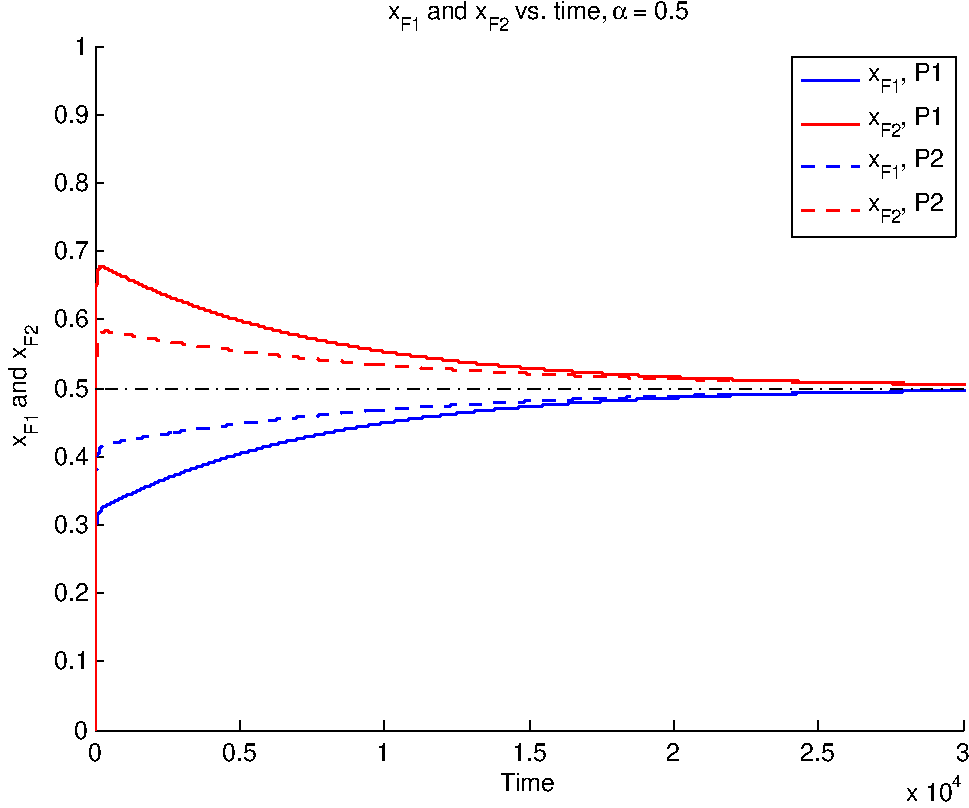
\includegraphics[width=7.2cm]{img/optim_conv_alpha05_lin.pdf}
                \label{fig:optim_objfct_comparison:alpha05_lin}
            }
    %       \: % espacement entre figures. \quad \;
            \subfigure[$\alpha = 0.5$, Log x axis.]
            {
                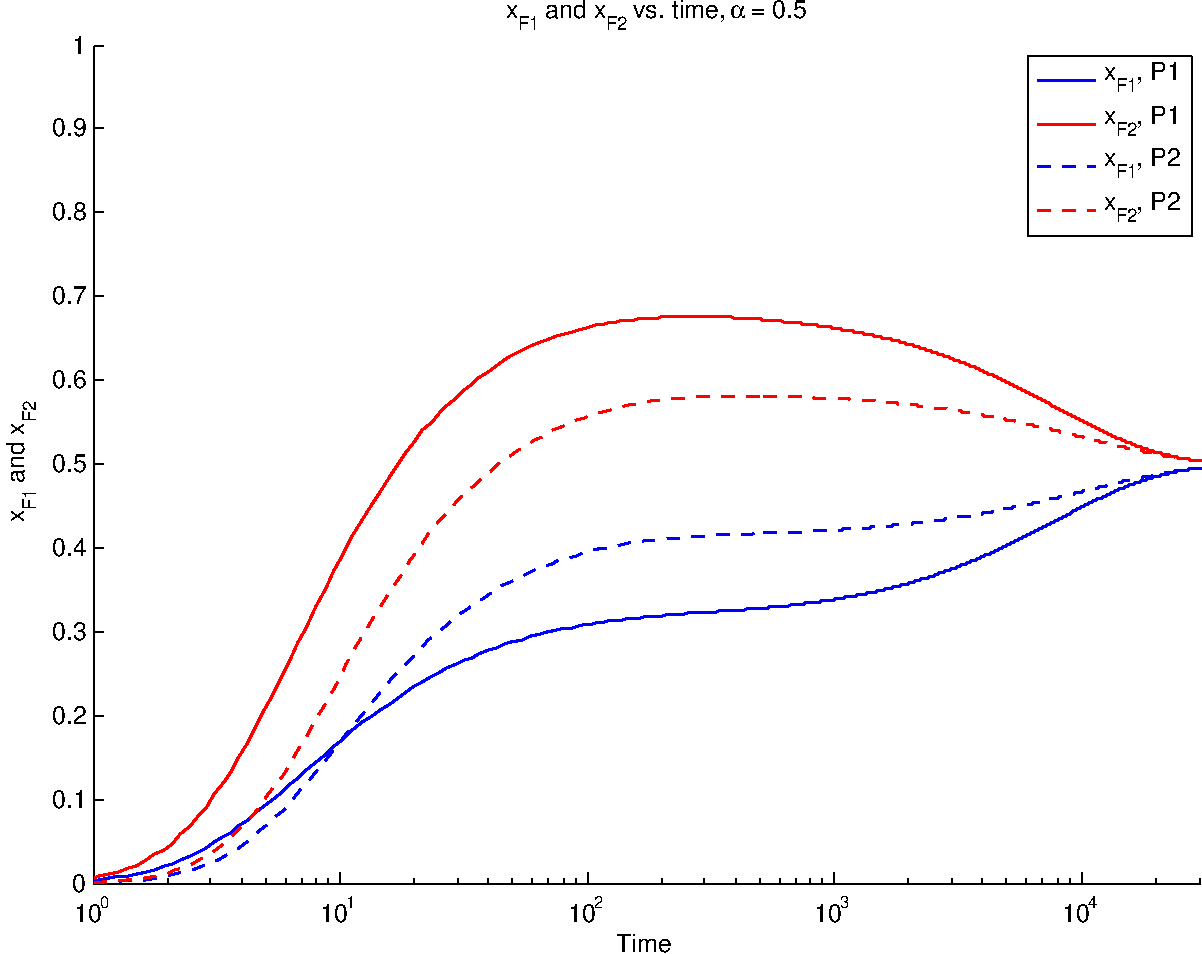
\includegraphics[width=7.2cm]{img/optim_conv_alpha05_log.pdf}
                \label{fig:optim_objfct_comparison:alpha05_log}
            }
    %       \: % espacement entre figures. \quad \;
            \subfigure[$\alpha = 0.9$, Linear x axis.]
            {
                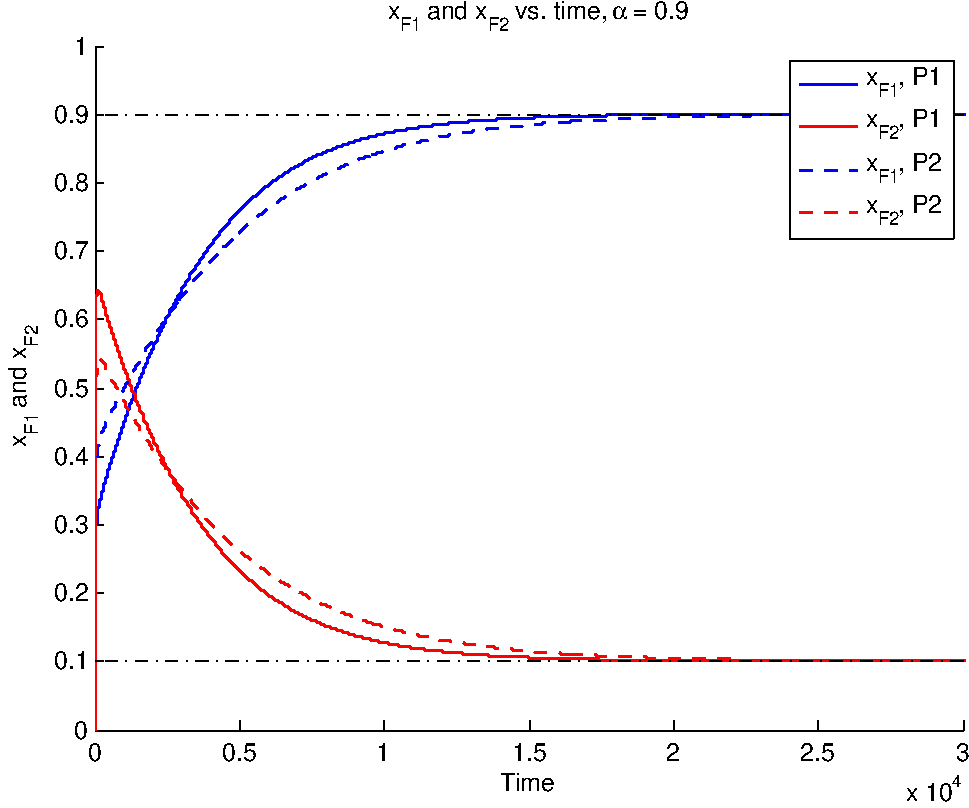
\includegraphics[width=7.2cm]{img/optim_conv_alpha09_lin.pdf}
                \label{fig:optim_objfct_comparison:alpha09_lin}
            }
    %       \: % espacement entre figures. \quad \;
            \subfigure[$\alpha = 0.9$, Log x axis.]
            {
                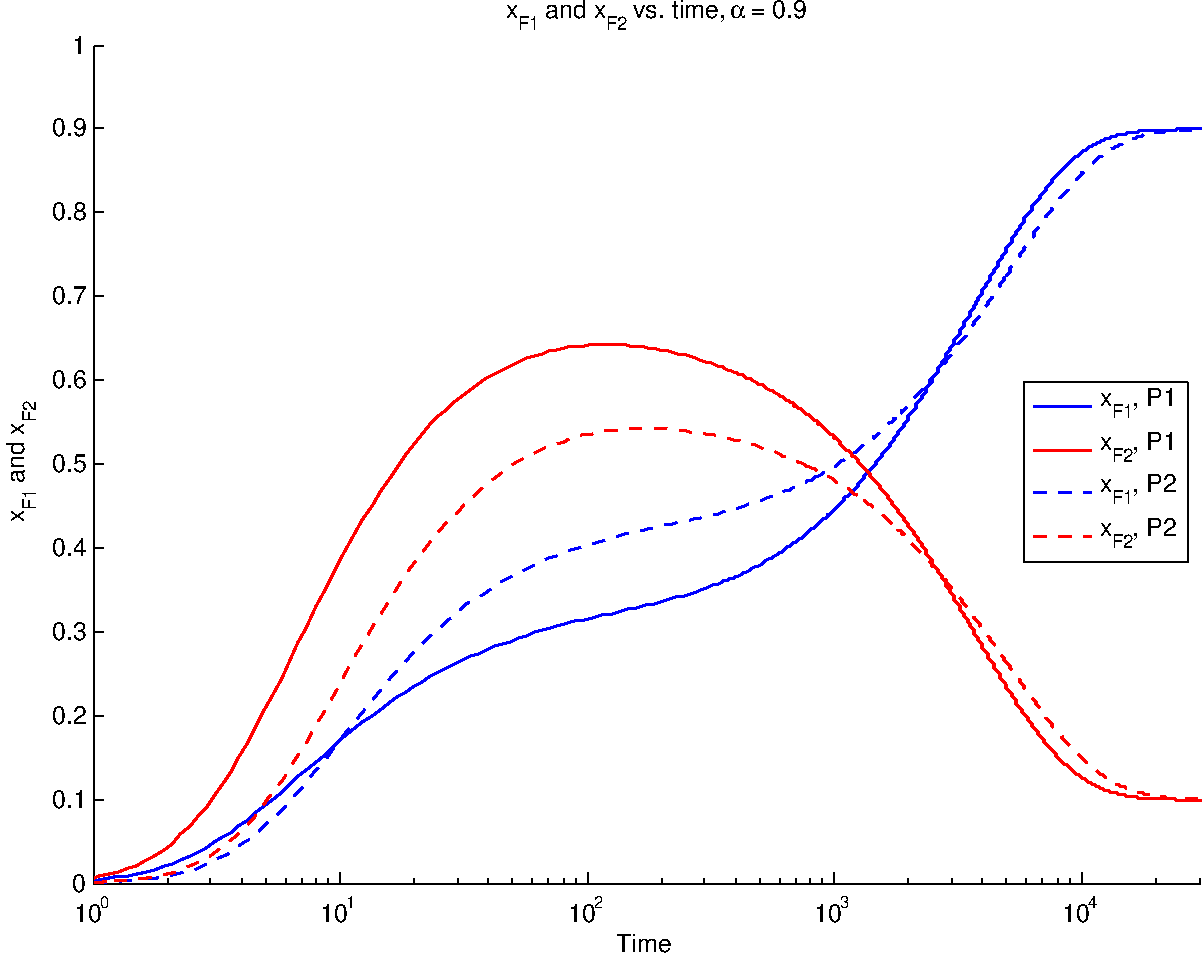
\includegraphics[width=7.2cm]{img/optim_conv_alpha09_log.pdf}
                \label{fig:optim_objfct_comparison:alpha09_log}
            }
            \caption{Comparison between the two objective functions P1 and P2, as well as difference in behavior when showed with semi-logarithmic x axis.}
        \label{fig:optim_objfct_comparison} %Caption general
        \end{figure}

        We see that P1 is converging quicker than P2 to the equilibrium for $\alpha=0.1$ and $\alpha=0.9$, but is slower for $\alpha=0.5$. It is still unclear if it is only due to the values of the forward rates, as hypothesized. The overall speed of convergence is actually pretty slow, especially when trying to produce $50\%$ of both puzzles. This could be problematic, but is in fact linked to the global behavior of the system, as we show now.

        Looking at semi-logarithmic plots of the same data, we clearly see two regime of convergence:

        \begin{my_itemize}
            \item A quick convergence to an unique equilibria, independent of the chosen $\alpha$, till $t=10^2 s$. We hypothesize that this equilibrium depends on the network topology and forward rates.
            \item A ``redistribution'' regime starting from there, which makes the system converge to the final $\alpha$ desired. This regime is much slower than the first one. The final reactions with optimized rates only act during that regime.
        \end{my_itemize}

        If we think in the state space of final assemblies, it means that the system first converge quickly to its intrinsic equilibrium, and then moves around slowly due to the redistribution of final puzzles until it arrives to the desired equilibrium.

        This is a very interesting and quite counterintuitive result, as one might think that it would be best to go directly towards the desired equilibrium. The optimization process we use seems to point out that going quickly to the intrinsic equilibrium and then moving from there is a better strategy. Of course, this might be an artifact of the linear optimization we do, so a verification with another optimization process should be performed. This will be done in further works.

    % subsection comparison_between_objective_function_and_strategies (end)

        % \item The overall convergence to a desired equilibrium
        %
        % It means that the optimized way to converge to an equilibrium is the following:
        %   \begin{my_itemize}
        %       \item First converge as quickly as possible towards the equilibrium given by the system without backward reactions.
        %       \item The backward reactions starts their full effect when the number of final puzzles is big enough.
        %       \item The system slowly converge.
        %   \end{my_itemize}

    \subsection{Online adaptation of the desired final puzzles ratio} % (fold)
    \label{sub:online_adaptation_of_the_desired_final_puzzles_ratio}
        We finish by showing the application of the rate optimization to the ``green manufacturing'' process shortly presented in Section~\ref{sec:definition_of_the_puzzle_test_case}. A ``green manufacturing'' process is a direct application of the flexibility offered by a non-specific assembly task. In that process, we reuse finished products (in our case, final puzzles) in order to create new products, depending on the current demand. We ``recycle'' the products into new ones. This is possible because our system possess the capabilities to create both products, and because we fix what it is supposed to create by optimizing the rates of assembly as shown in this chapter.

        We show such an example of online adaptation to a new goal, by simulating the following experiment:

        \begin{my_itemize}
            \item Through all this experiment, we use the optimized goals under objective function P1, see Table~\ref{tab:optimized_rates_p1} and Figure~\ref{fig:img_optimized_rates_alpha_p1}.
            \item We initialize the system with a first goal of a $60\%$ ratio of final puzzle F2. We let the system run till $t_1 = 1000 s$.
            \item We change the rates to the one optimized to create a ratio of $99\%$ final puzzle F1. We let the system run till $t_2 = 6000 s$.
            \item We change the rates to a goal of $99\%$ of final puzzle F2 ($\alpha=0.01$). We let the system run till $t_3 = 11000 s$.
            \item We change for the last time the rates for a goal of $50\%$ of each final puzzle. We let the system run till $t_4 = 21000 s$.
        \end{my_itemize}

        The result is shown in Figure~\ref{fig:optim_online_adaptation}. We see that the system is capable of adapting smoothly to abrupt new commands in the desired targets. It attains the desired ratio when converged. The convergence time is pretty slow when approaching the desired ratio, yet early change occurs quickly. The target of $50\%$ of both puzzles is slower to attain.

    \begin{figure}[h!]
        \centering
            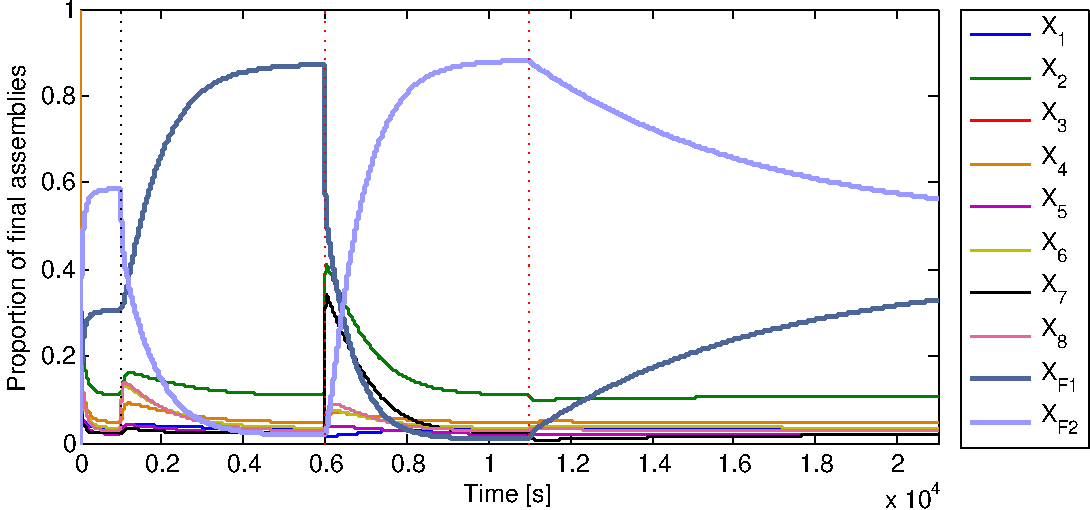
\includegraphics[width=13cm]{img/optim_online_adaptation.pdf}
        \caption{Change of reaction rates during an experiment. System adapts smoothly to the new equilibrium. Modifications of rates are shown with dotted vertical lines. First goal is 60\% of F2, second is 100\% of F1, third is 100\% of F2 and fourth is 50\% of each.}
        \label{fig:optim_online_adaptation}
    \end{figure}

    A good result is the speed of adaptation to new commands, and the strong redistribution effect of commands asking for near $100\%$ ratios. We think it is also possible to design a control policy stabilizing quicker to a slow target ($50\%$ for example) by switching between a $100\%$ F1 and a $100\%$ F2 command, slowly damping the oscillations till we attain the desired distribution. This is a similar approach to the one shown in \cite{Julius:2007p4774, Julius:2008p4775} for the control of switching in \textit{E. Coli}. More tests are still necessary to assess the validity of this process, but the behavior we obtain already offers us a large variety of adaptable behaviors.

    % subsection inline_adaptation_of_the_desired_final_puzzles_ratio (end)

% section results_and_limitations (end)




\section{Beyond control, direct optimization of the plan?} % (fold)
\label{sec:beyond_control_direct_optimization_of_the_plan_}
    Can our optimization scheme optimize directly a set of assembly plans? We addressed that problem in Section~\ref{sec:considerations_on_the_assembly_plan}, while speaking about the optimal plans. Given optimized rates, it is possible to see if some reactions are promoted or deactivated. This corresponds to a continuous optimization of the assembly plan, effective while the system is behaving. We will alter our model in order to test that hypothesis.

    We add new assembly steps to create additional pathways to the final assemblies. In addition to plans shown in Figures~\ref{fig:assembly_plans}, we add two new plans, that reuse parts of the old ones, see Figures~\ref{fig:assembly_plans_added}. The new assembly steps are shown in boldface. We call those new plans ``linear plans'', as they assemble one piece at a time without parallel processes. Our goal is to see how the algorithm treats these new pathways, more precisely if it ``shuts down'' the ones which are not optimal or useful.

    \begin{figure}[h!]
        \centering
        \subfigure[New added first final puzzle plan]
        {
            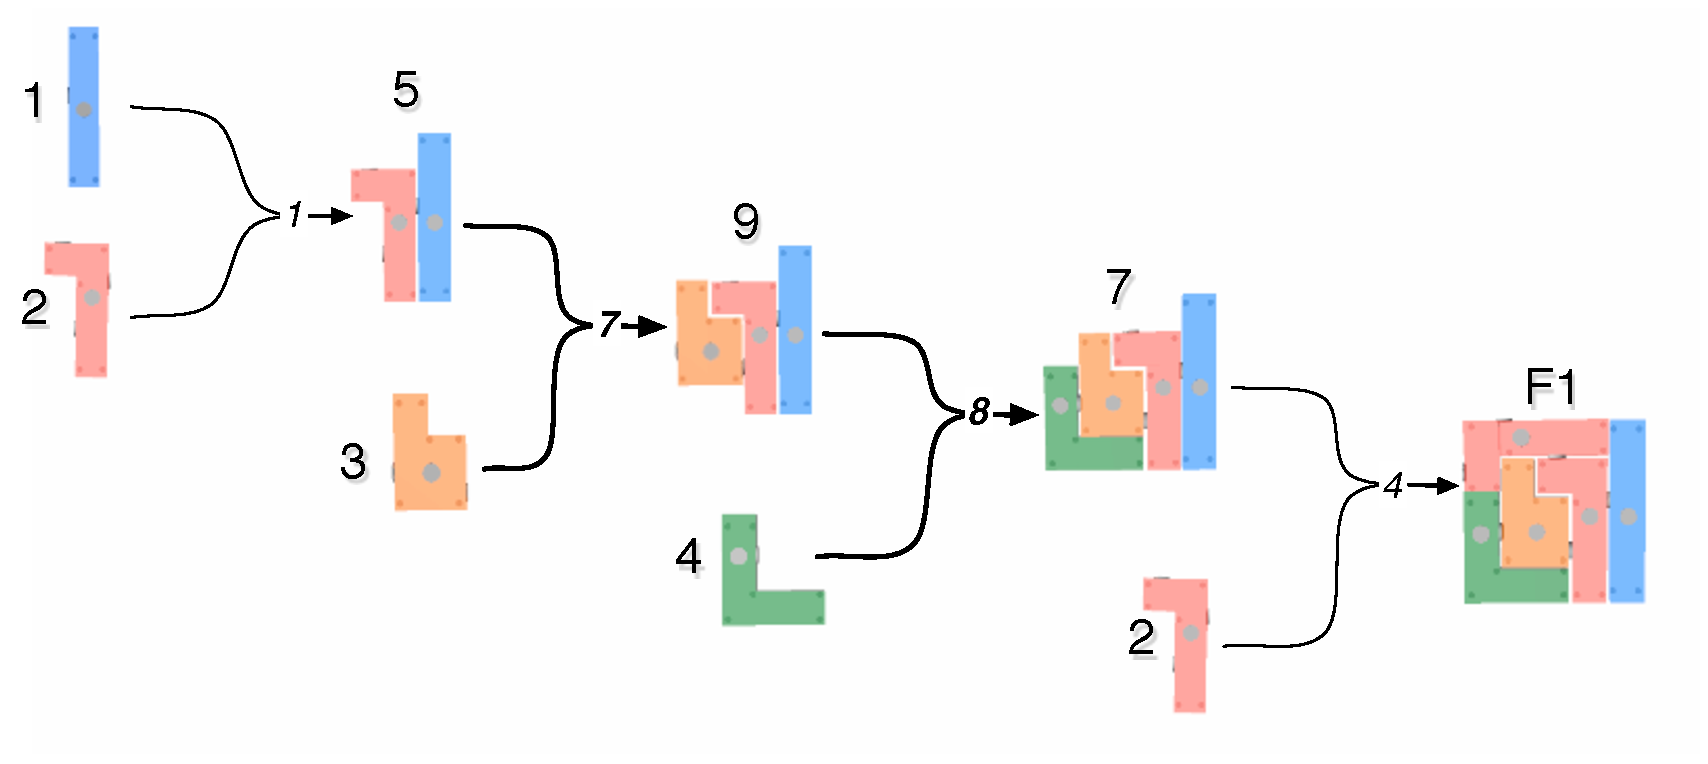
\includegraphics[width=11cm]{img/assembly_plan_f1_added.pdf}
            \label{fig:assembly_plans_added:f1}
        }
        \; % espacement entre figures. \quad \;
        \subfigure[New added second final puzzle plan]
        {
            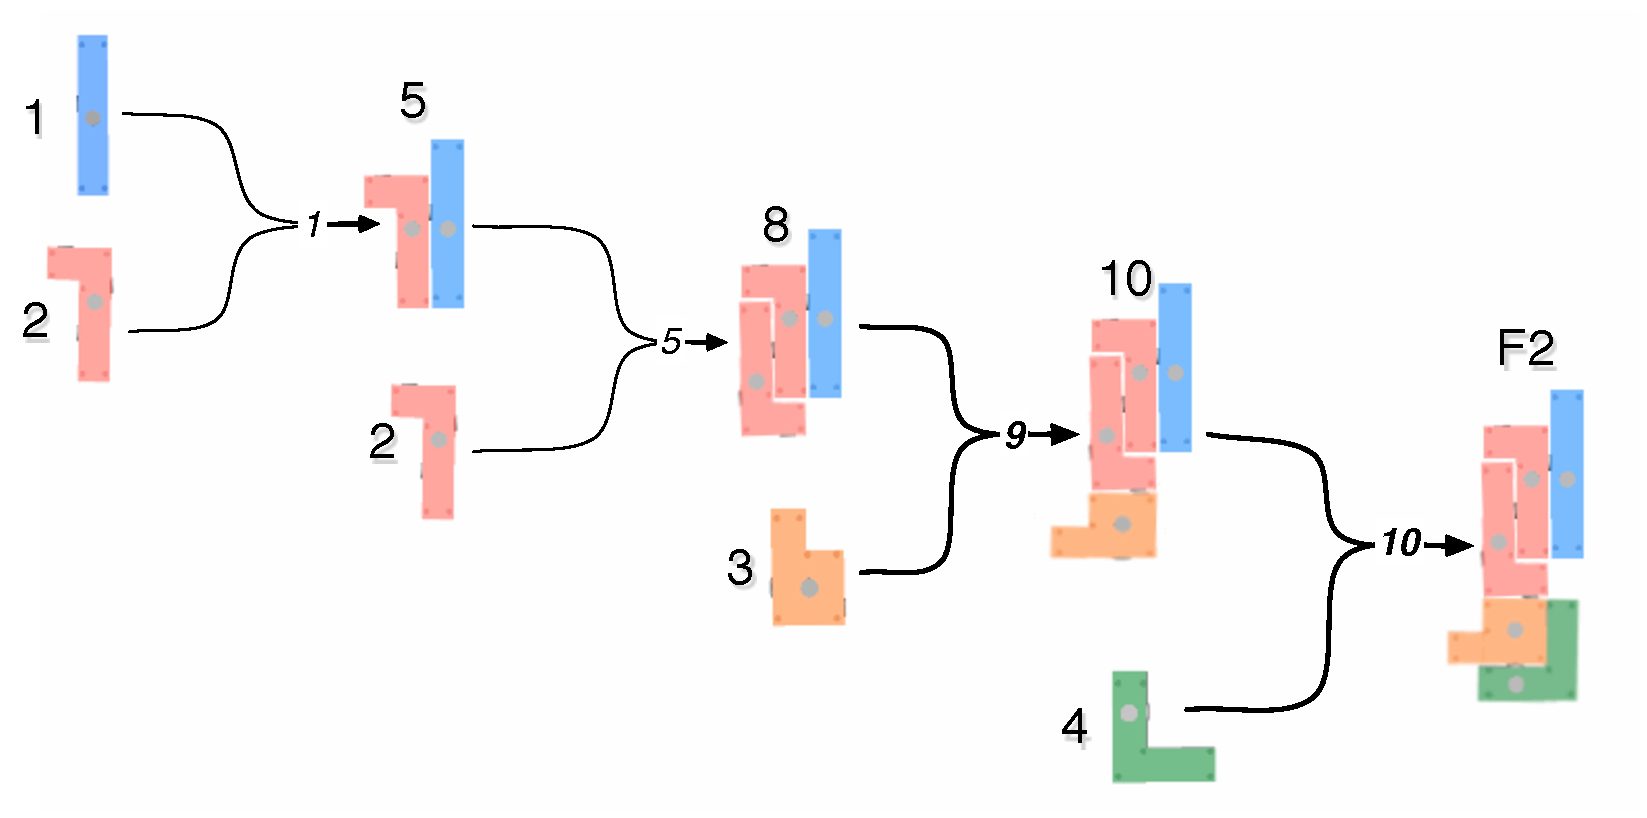
\includegraphics[width=11cm]{img/assembly_plan_f2_added.pdf}
            \label{fig:assembly_plans_added:f2}
        }
        \caption{New plans created by adding 4 new assembly steps, written in boldface. We call those plans the ``linear plans'', as they act by assembling one piece after another without parallel processes.}
    \label{fig:assembly_plans_added} %Cation general
    \end{figure}

    The 4 added assembly steps translate into the following reactions to be added to the set \eqref{eq:modified_system:reactions}:
    \begin{eqnarray}
        X_3 + X_5 ~~{\mathop{\rightleftharpoons}_{k_{7}^-}^{k_{7}^+}}~~ X_{9} & \quad & X_3 + X_8 ~~{\mathop{\rightleftharpoons}_{k_{9}^-}^{k_{9}^+}}~~ X_{10} \nonumber \\
        X_4 + X_{9} ~~{\mathop{\rightleftharpoons}_{k_{8}^-}^{k_{8}^+}}~~ X_7 & & X_4 + X_{10} ~~{\mathop{\rightleftharpoons}_{k_{10}^-}^{k_{10}^+}}~~ X_{F2}
    \label{eq:reactionsExp}
    \end{eqnarray}

    With these added reactions, the ODE equations for the system are:

    \begin{equation} \label{eq:ODEequationsExp}
        \left\lbrace\begin{array}{lll}
            \dot{x}_1 &=& - k_1^+ x_1 x_2 + k_1^- x_5    \\
            \dot{x}_2 &=& - k_1^+ x_1 x_2 - k_5^+ x_2 x_5 - k_4^+ x_2 x_7 + k_1^- x_5 + k_{5}^- x_8 + k_4^- x_{F1}  \\
            \dot{x}_3 &=& - k_2^+ x_3 x_4 + k_2^- x_6 - k_{7}^+ x_3 x_5 + k_{7}^- x_{9} - k_{9}^+ x_3 x_8 + k_{9}^- x_{10}  \\
            \dot{x}_4 &=& - k_2^+ x_3 x_4 + k_2^- x_6 - k_{8}^+ x_4 x_9 + k_{8}^- x_{7} - k_{10}^+ x_4 x_{10} + k_{10}^- x_{F2}  \\
            \dot{x}_5 &=&   k_1^+ x_1 x_2 - k_1^- x_5 - k_3^+ x_5 x_6 + k_3^- x_7 - k_5^+ x_2 x_5 \\
             &  & + k_{5}^- x_8 - k_{7}^+ x_3 x_5 + k_{7}^- x_{9}  \\
            \dot{x}_6 &=&   k_2^+ x_3 x_4 - k_2^- x_6 - k_3^+ x_5 x_6 + k_3^- x_7 - k_{6}^+ x_6 x_8 + k_{6}^- x_{F2}  \\
            \dot{x}_7 &=&   k_3^+ x_5 x_6 - k_3^- x_7 - k_4^+ x_2 x_7 + k_4^- x_{F1} + k_{8}^+ x_4 x_9 - k_{8}^- x_{7}   \\
            \dot{x}_8 &=&   k_5^+ x_2 x_5 - k_{5}^- x_8 - k_{6}^+ x_6 x_8 + k_{6}^- x_{F2} - k_{9}^+ x_3 x_8 + k_{9}^- x_{10} \\
            \dot{x}_9 &=&   k_{7}^+ x_3 x_5 - k_{7}^- x_{9} - k_{8}^+ x_4 x_{9} + k_{8}^- x_{7}   \\
            \dot{x}_{10} &=& k_{9}^+ x_3 x_8 - k_{9}^- x_{10} - k_{10}^+ x_4 x_{10} + k_{10}^- x_{F2}   \\
            \dot{x}_{F1} &=& k_4^+ x_2 x_7 - k_4^- x_{F1}  \\
            \dot{x}_{F2} &=& k_{6}^+ x_6 x_8 - k_{6}^- x_{F2} + k_{10}^+ x_4 x_{10} - k_{10}^- x_{F2} \\
        \end{array}
        \right.
    \end{equation}

    Like system \eqref{eq:ODEequations}, this system can be written in
    the form \eqref{eq:matrixODE}.  In this case, the vector of
    complexes is defined as

    \begin{eqnarray}
        \mathbf{y(x)} = &&[x_1 x_2,~x_5,~x_3 x_4,~x_6,~x_2 x_7,~ x_{F1},~ x_5
        x_6,~ x_7,~ x_2 x_5, \nonumber \\
        && x_8,~ x_6 x_8,~ x_{F2},~ x_3 x_5,~ x_{9},~ x_4 x_{9},~ x_3
        x_8,~ x_{10},~ x_4 x_{10}]^T~. \label{eq:yExp}
    \end{eqnarray}

    %[diff labels for S, K, y in expanded system?]

    One set of conservation constraints on the piece quantities in this system is:
    \begin{equation}\label{eq:consExp}
        \left\lbrace\begin{array}{lll}
            x_1+x_5+x_7+x_8+x_{F1}+x_{F2}+x_{9}+x_{10} &=& N_5 \\
            x_2+x_5+x_7+2 x_8+2 x_{F1}+2 x_{F2}+x_{9}+2 x_{10} &=& N_6 \\
            x_3+x_6+x_7+x_{F1}+x_{F2}+x_{9}+x_{10} &=& N_7\\
            x_4 + x_6 + x_7 + x_{F1} + x_{F2} &=& N_8
        \end{array}
        \right.
    \end{equation}

    where $N_i$, $i=5,...,8$, are computed from the initial piece
    quantities.

    \subsection{Optimized rates and induced effective plan} % (fold)
    \label{sub:optimized_rates}
        We apply our optimization procedure with Problem P1 and P2 as before. The results for the convergence are shown in Figure~\ref{fig:exp_optim_objfct_comparison}. As Problem P2 is quicker in general and shows more interest dynamics, we will only study it for the rest of this section.

            \begin{figure}[h!]
                %\centering
                \subfigure[$\alpha = 0.1$, Log x axis.]
                {
                    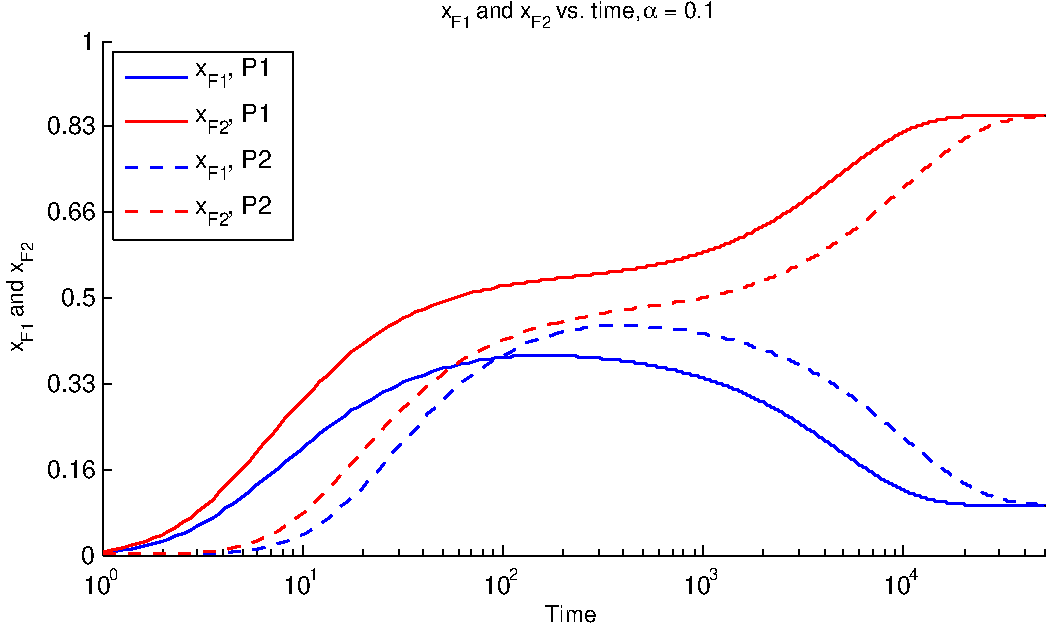
\includegraphics[width=7.2cm]{img/optim_exp_conv_alpha01.pdf}
                    \label{fig:exp_optim_objfct_comparison:alpha01_log}
                }
        %       \: % espacement entre figures. \quad \;
                \subfigure[$\alpha = 0.5$, Log x axis.]
                {
                    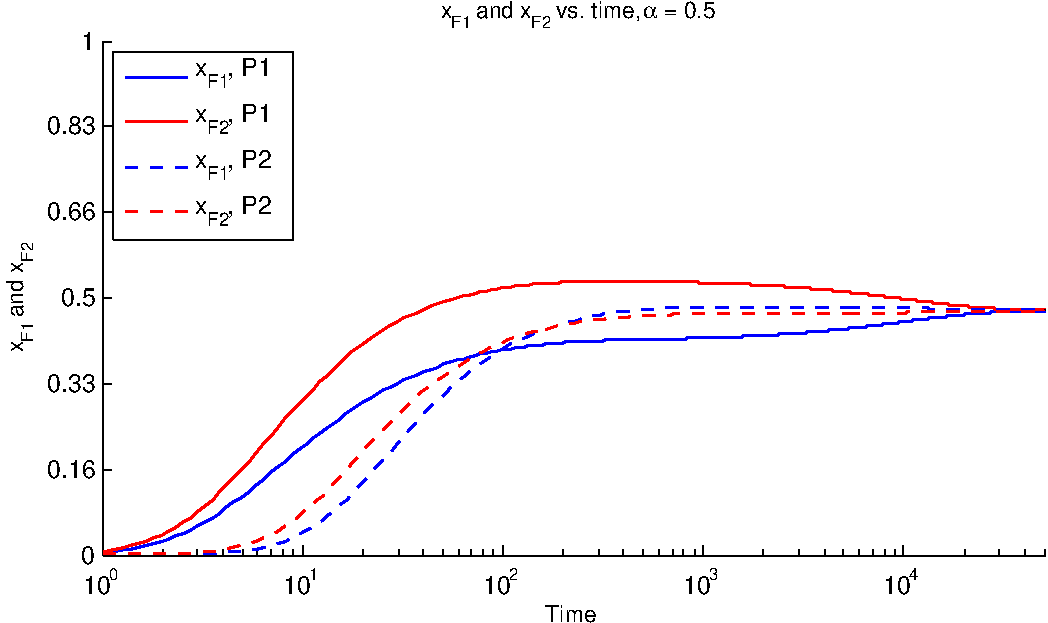
\includegraphics[width=7.2cm]{img/optim_exp_conv_alpha05.pdf}
                    \label{fig:exp_optim_objfct_comparison:alpha05_log}
                }
        %       \: % espacement entre figures. \quad \;
                \subfigure[$\alpha = 0.9$, Log x axis.]
                {
                    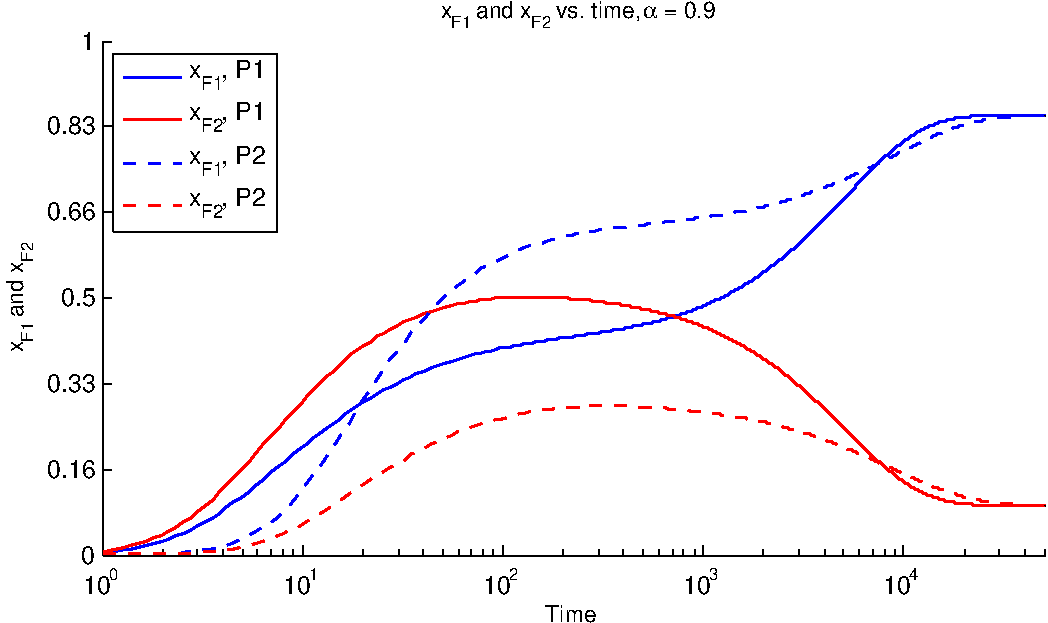
\includegraphics[width=7.2cm]{img/optim_exp_conv_alpha09.pdf}
                    \label{fig:exp_optim_objfct_comparison:alpha09_log}
                }
                \caption{Expanded system. Comparison between the two objective functions P1 and P2 when showed with semi-logarithmic x axis.}
            \label{fig:exp_optim_objfct_comparison} %Caption general
            \end{figure}

        The resulting probabilities $p_i^+, p_i^-$ for problem P2 are nearly all continuously varying. The only exceptions are $p_3^+$, $p_6^+$ and $p_9^+$ which are all at $1.0$. The variation of the rates for the values of $\alpha$ are shown in Figure~\ref{fig:exp_optim_varying_rates}.

        \begin{figure}[h!]
            \centering
            \subfigure[Forward rates varying continuously]
            {
                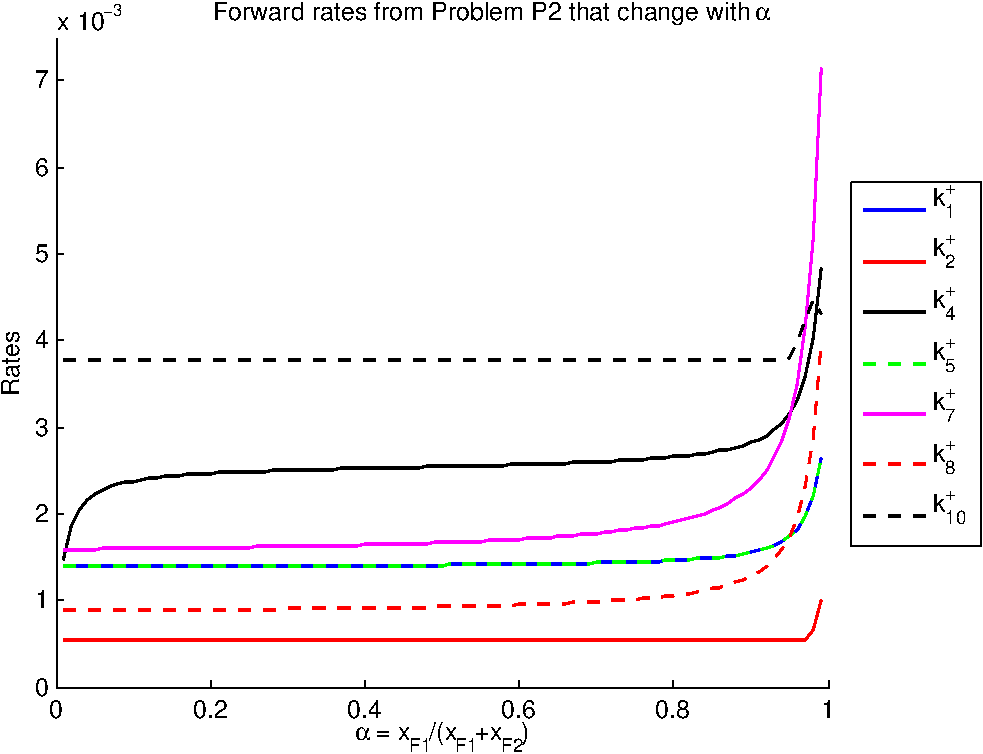
\includegraphics[width=10cm]{img/optim_exp_forward_rates.pdf}
                \label{fig:exp_optim_varying_rates:forward}
            }
    %       \: % espacement entre figures. \quad \;
            \subfigure[Backward rates varying continuously]
            {
                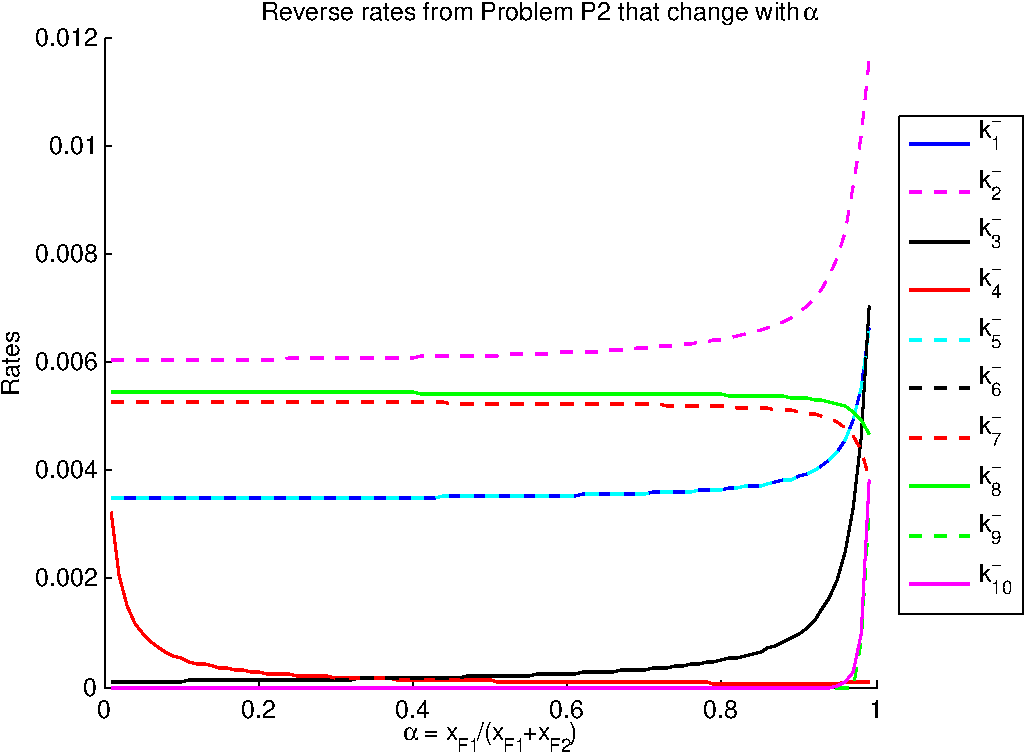
\includegraphics[width=10cm]{img/optim_exp_backward_rates.pdf}
                \label{fig:exp_optim_varying_rates:backward}
            }
    %       \: % espacement entre figures. \quad \;
            \caption{Optimized rates of expanded system under problem P2, for $\alpha \in \{0.1, 0.9\}$. Remark: $k_6^-$ curve is merged with $k_3^-$.}
        \label{fig:exp_optim_varying_rates} %Caption general
        \end{figure}

        Looking at the values of the rates at specific positions, we can make observation on the actual plan promoted by the optimization. The reactions, though still present, will be promoted or deactivated when their corresponding forward and backward rates are modified. This corresponds to a continuous optimization of the plan, in contrast with a discrete optimization performed by Klavins\cite{Klavins:2007p2600}.

        In general, the value of the rates show the following hierarchy between reactions and pathways:
        \begin{itemize}
            \item $k_2^+$ is small and $k_2^-$ is big compared to other rates. This deactivates Reaction 2.
            \item To compensate the absence of piece 6, the linear pathways represented by reactions 7 and 8 for F1 and reactions 9 and 10 for F2 are really active.
            \item The small amount of pieces 6 that would result from breaking of assemblies are quickly reuse via the reactions 3 and 6, which have of full forward rate, or destroyed by the backward rate of reaction 2.
        \end{itemize}

        We see three different regimes for the rates, and the resulting continuous assembly plans:
        \begin{my_enumerate}
            \item Near $\alpha=0.1$, the only changing rates are $k_4^+$ and $k_4^-$. They are changing toward a deactivation of Reaction 4, which is the only one creating F1 puzzles. The network then automatically tends to create more F2 puzzles, which seems to be a constant characteristic of the system we are studying.
            \item Between $\alpha=0.2$ and $\alpha = 0.8$, the rates $k_4^+$ and $k_6^-$ seems to have to most effect. They act by promoting the creation of F1 and slowing the creation of F2. During that period, the networks tends to produce a $50\%$ ratio by itself, as shown by the convergence profile in Figure~\ref{fig:exp_optim_objfct_comparison:alpha05_log}: the first convergence arrives close to a $50\%$, no redistribution is needed (to compare with Figure~\ref{fig:optim_objfct_comparison:alpha05_log} of the previous system)
            \item Near $\alpha = 0.9$, the behavior changes dramatically. Reactions 7, 8 and 4, leading to the creation of F1 are promoted extensively (increase in forward rate, decrease in backward rate). At the same moment, reactions 6 and 10, creating F2, are deactivated. This promotes the creation of F1 puzzles.
        \end{my_enumerate}

        We see then that this optimization works with these general tendencies:

        \begin{my_itemize}
            \item Remove assembly 6 from the possible pool of pieces, to liberate all initial pieces for other reactions. This means removing the initial plans we were using an use the new introduced one, see Figure~\ref{fig:assembly_plans_added}
            \item Use the linear steps to create the final puzzles. This is a counter-intuitive results, but it may be linked to an added flexibility with having a large pool of initial pieces, that can be used at precise assembly steps without temporal dependences between reactions.
            \item Modify the reactions leading to the final assemblies to change the ratio, and do not touch the ``general'' part of the system. This is in agreement with the behavior we observed in last section.
            \item As the system is more prone to create F2 than F1, it is easier to control the system in one direction than the other. To create a big ratio of F1, the overall behavior of the system is changed, leading to a nearly new plan. This plan correspond to the linear one we added in Figure~\ref{fig:assembly_plans_added:f1}.
        \end{my_itemize}

    % subsection optimized_rates (end)

    So in conclusion, it is possible to get insights into the kind of behaviors and continuous plans promoted by the optimization. The algorithm promoted the use of linear plans, with the addition of ``rewiring'' the system when the goal to attain is in contradiction with the intrinsic behavior of the system (e.g. to create the big ratio of F1).

    These results are not that intuitive, i.e. one would think that using parallel assembly steps is more efficient for the convergence time, yet comparing the convergence time seems to give credits to the optimization technique (e.g. for $\alpha = 0.5$, the convergence is much more efficient, whereas for $\alpha=0.1$ and $\alpha=0.9$ it is similar).
    However, it has to be checked that such an optimization would give similar results for a more complicated set of assembly plans.
% section beyond_control_direct_optimization_of_the_plan_ (end)
